\documentclass[useAMS,usenatbib,referee]{biom}

\usepackage{amsmath}
\usepackage[figuresright]{rotating}

\graphicspath{{include/}}

\def\bSig\mathbf{\Sigma}
\newcommand{\VS}{V\&S}
\newcommand{\tr}{\mbox{tr}}

\newcommand{\blind}{1} % 0 = not blind, 1 = blind

%\newcommand{\Stan}{{\tt Stan}}
\newcommand{\Stan}{Stan}
\newcommand{\RStan}{{\tt RStan}}
\newcommand{\edgeR}{{\tt edgeR}}
\newcommand{\baySeq}{{\tt baySeq}}
\newcommand{\ShrinkBayes}{{\tt ShrinkBayes}}
\newcommand{\RNAseq}{RNA-seq}

%\renewcommand{\gamma}{c}


\title{Empirical Bayes analysis of \RNAseq{} data for detection of gene expression heterosis}

\if0\blind{
\author{Jarad Niemi$^*$\email{niemi@iastate.edu}, 
Eric Mittman, 
Will Landau, and 
Dan Nettleton \\
Department of Statistics, Iowa State University, Ames, Iowa, U.S.A.}
} \fi

\begin{document}

\date{{\it Received July} 2015} 

\pagerange{\pageref{firstpage}--\pageref{lastpage}} 
\volume{VV}
\pubyear{YYYY}
\artmonth{MM}
\doi{x}

\label{firstpage}

\begin{abstract}
An important type of heterosis, known as hybrid vigor, refers to the enhancements in the phenotype of hybrid progeny relative to their inbred parents. Although the heterosis phenomenon is extensively utilized in agriculture, the molecular basis of heterosis is still largely unknown. In an effort to understand phenotypic heterosis at the molecular level, researchers are measuring transcript abundance levels of thousands of genes in parental inbred lines and their hybrid offspring using RNA sequencing (\RNAseq{}) technology.  The resulting data allow researchers to search for evidence of gene expression heterosis as one potential molecular mechanism underlying heterosis of agriculturally important traits.  The null hypotheses of greatest interest in testing for gene expression heterosis are composite null hypotheses that are difficult to test with standard statistical approaches for \RNAseq{} analysis. To address these shortcomings, we develop a hierarchical negative binomial model and draw inferences using a computationally tractable empirical Bayes approach to inference. We demonstrate improvements over alternative methods via a simulation study based on a maize experiment and then analyze that maize experiment with our newly proposed methodology. 
% This article has supplementary material online.
\end{abstract}

\begin{keywords}
Hierarchical model; Negative binomial; \RNAseq{}; Bayesian LASSO; Parallel computing; \Stan{}.
\end{keywords}

\maketitle

%  A maximum of six (6) tables or figures combined is often required.''

\section{Introduction}
\label{s:intro}

Heterosis exists when the expected value of a hybrid phenotype differs from the average of the expected phenotypic values of the hybrid's parents.  The most interesting and useful form of heterosis, known as hybrid vigor, occurs when hybrid progeny display a mean phenotype that is superior to  both parental phenotypic means.  This heterosis phenomenon was scientifically documented in plants by \cite{darwin1876effects} and has long been used to improve agricultural production. One classic example involves hybrid maize offspring that are taller, faster to mature, and yield considerably more grain than their inbred parents \citep{hallauer1981quantitative, hallauer2010quantitative}.

Depending on whether large or small values of a phenotype are favorable, hybrid vigor can occur if the mean phenotype of a hybrid is greater than both parental means or less than both parental means. We refer to the former as high-parent heterosis (HPH) and the latter as low-parent heterosis (LPH). Note that heterosis, HPH, and LPH are similar to the quantitative genetics concepts of dominance, heterosis, and underdominance.  However, the various forms of dominance are usually reserved for describing the association of mean phenotype with homozygous and heterozygous genotypes at a single genetic locus.  Heterosis involves a comparison of inbreds (simultaneously homozygous at many loci) and hybrids (simultaneously heterozygous at many loci).  For simplicity, throughout the remainder of the article, we will use the term \emph{extreme heterosis} to describe the situation where the hybrid mean is more extreme than the parental means, i.e. we say there is heterosis if and only if either HPH or LPH holds.

Despite intensive study and successful use of heterosis in agriculture, the basic molecular genetic mechanisms remain poorly understood \citep{chen2013genomic}. One potential explanation, known as gene expression heterosis, is enhanced expression of one or more genes in hybrids compared to their inbred parents.  Gene expression heterosis has been investigated in maize by \cite{swanson2006all} and \cite{springer2007allelic} and is conceptually depicted in the right column of Figure 1b in  \cite{chen2013genomic}.

Recently, \cite{ji2014estimation} introduced an approach to assess gene expression heterosis using microarray data under the assumption that these data are continuous. They built a normal hierarchical model for microarray measurements of transcript abundance that allows borrowing of information across genes to estimate means and variances. They introduced an empirical Bayes framework that first estimates model hyperparameters, then estimates the posterior distribution for gene-specific parameters conditional on those hyperparameters, and finally computes heterosis probabilities based on integrals of regions under this posterior. This development was necessary due to the composite null hypotheses in tests for heterosis. These hypotheses, which many available methods do not fully accommodate, remain a challenge in the transition from continuous measurements of transcript abundance to count-based measurements that arise from RNA sequencing (\RNAseq{}) technology. Building on the work of \citeauthor{ji2014estimation} with the normal data model, we construct a hierarchical model based on a negative binomial data model. We also utilize an empirical Bayes approach to obtain estimates of the hyperparameters and the posterior distributions for the gene-specific parameters conditional on those hyperparameters. 

The remainder of the paper proceeds as follows. Section \ref{s:method} presents the proposed hierarchical model, an empirical Bayes method of estimating the parameters, and the calculation of posterior probabilities of heterosis. Section \ref{s:simulation} presents a simulation study based on a maize experiment and compares our approach to alternative methods. Section \ref{s:maize} analyzes a maize experiment where phenotypic heterosis is well established and identifies genes demonstrating expression heterosis. The data and code necessary to perform this analysis are available in the Supplemental Material. Section \ref{s:discussion} summarizes the work and suggests directions for future research.


\section{Empirical Bayes identification of gene expression heterosis from \RNAseq{} read counts}
\label{s:method}

We consider an RNA sequencing (\RNAseq{}) experiment that involves at least three genetic varieties: two parental varieties (P1 and P2) and a cross between these two varieties called the hybrid (H). For each variety, replicate RNA samples are isolated and assessed for quality. Complementary DNA (cDNA) libraries, consisting of short cDNA fragments derived from RNA, are constructed. Then, next generation sequencing technology is used to determine the \emph{reads}, or nucleotide sequences, in the cDNA libraries. These reads are processed using bioinformatic algorithms to match the reads to genes, or specific gene transcripts, exons, microRNAs, etc. The results of read processing are summarized by a gene $\times$ sample matrix of counts. See \cite{datta2014statistical} for more details on \RNAseq{} experiments and data from a statistical perspective, and see \cite{paschold2012complementation} for the biological background behind the use of \RNAseq{} to study gene expression heterosis.

To use \RNAseq{} counts to identify genes displaying expression heterosis, we build a hierarchical model to borrow information across gene-variety means and across gene-specific overdispersion parameters, estimate the hyperparameters using an empirical Bayes procedure, and calculate empirical Bayes posterior probabilities for extreme heterosis. 


\subsection{Hierarchical model for \RNAseq{} counts}
\label{s:model}

Let $Y_{gvi}$ be the count for gene $g=1,\ldots,G$, variety $v=1,\ldots,V$, and replicate $i=1,\ldots,n_v$.  We assume
\begin{equation} 
Y_{gvi} \stackrel{ind}{\sim} \mbox{NB}\left(e^{\mu_{gv}+\gamma_{vi}},e^{\psi_g}\right), 
\label{e:data}
\end{equation}
where NB$(\xi,e^\psi)$ indicates a negative binomial distribution with expectation $\xi$ and variance $\xi+e^\psi\xi^2$, and $ind$ indicates the observations are conditionally independent.  As shown in equation \eqref{e:data}, our data model involves gene-specific overdispersion $\psi_g$ and a mean that depends on the gene-variety combination through $\mu_{gv}$ and on the sample though  $\gamma_{vi}$.  The $\mu_{gv}$ terms are of primary scientific interest; the $\gamma_{vi}$ terms are normalization factors that account for differences in the thoroughness of sequencing from sample to sample. 

Following \cite{ji2014estimation}, we reparameterize the gene-variety mean structure into the gene-specific parental average ($\phi_g$), half-parental difference ($\alpha_g$), and hybrid effect ($\delta_g$). For our heterosis study where $V=3$, we let $v=1,2$ indicate the two parental varieties and $v=3$ indicate the hybrid. The reparameterization is  
\[ \phi_g = \frac{\mu_{g1}+\mu_{g2}}{2}, \quad 
\alpha_g = \frac{\mu_{g1}-\mu_{g2}}{2}, \quad \mbox{and} \quad
\delta_g = \phi_g-\mu_{g3}. \]

We assume a hierarchical model for the gene-specific mean parameters and overdispersion parameters. Initially, we assume the parental averages, half-parental differences, hybrid effect, and overdispersion parameters follow normal distributions, i.e.
\[ 
%\gamma_{vi} \stackrel{ind}{\sim} N(0,\sigma_\gamma^2), \quad 
\phi_g \stackrel{ind}{\sim} N(\eta_\phi, \sigma_\phi^2), \,
\alpha_g \stackrel{ind}{\sim} N(\eta_\alpha, \sigma_\alpha^2), \,
\delta_g \stackrel{ind}{\sim} N(\eta_\delta, \sigma_\delta^2), \, \mbox{ and } \,
\psi_g \stackrel{ind}{\sim} N(\eta_\psi,\sigma_\psi^2). 
\]
Empirical plots of estimated values of $\alpha_g$ and $\delta_g$ for our maize data set (described in Section \ref{s:maize}) suggest that the distribution of these parameters are more peaked near zero and have heavier tails than a normal distribution allows. For differential expression between the two parental phenotypes, we would expect many genes to have small effects and only a few genes to have relatively large effects. For these many genes with small effects, we might expect the hybrid to act similar to its parents and therefore also have many genes where the hybrid effect is small and only a few genes where this hybrid effect is large. For these reasons, we also assessed Laplace (or double exponential) distributions for the half-parental difference and hybrid effect and thus implement a Bayesian LASSO \citep{park2008bayesian,hans2009bayesian}, i.e. 
\[ 
\alpha_g \stackrel{ind}{\sim} La(\eta_\alpha, \sigma_\alpha) \qquad \mbox{and} \qquad
\delta_g \stackrel{ind}{\sim} La(\eta_\delta, \sigma_\delta) 
\]
where $\alpha\sim La(\eta,\sigma)$ has a probability density function given by $La(\alpha;\eta,\sigma) = \exp(-|\alpha-\eta|/\sigma)/2\sigma$ with expectation $\eta$ and variance $2\sigma^2$. Whether using normal or Laplace distributions, we assume \emph{a priori} independence amongst the parental averages, half parental differences, hybrid effects, and overdispersion parameters.

\subsection{Empirical Bayes}
\label{s:ebayes}

Initial attempts to perform a fully Bayesian analysis via Markov chain Monte Carlo (MCMC) failed due to high computational costs and poor mixing in the resulting chains. For example, we implemented the model in the statistical software \Stan{} (discussed at the end of this section), ran the MCMC on a simulated data set with 10,000 genes for 2 months on a state-of-the-art linux server, and obtained potential scale reduction factors that suggested we would need to run at least ten times as long to obtain convergence. Although there are certainly improvements that could be made to decrease computational costs and improve mixing, we opted for an empirical Bayes approach. This approach may be a reasonable approximation to a fully Bayesian approach when estimating models with large numbers of genes as the posterior distributions for the hyperparameters may be tightly peaked. 

We categorize the parameters of the model in Section \ref{s:model} into gene-specific parameters $\theta = (\theta_1,\ldots,\theta_G)$ where $\theta_g = (\phi_g,\alpha_g,\delta_g,\psi_g)$, normalization factors $\gamma = (\gamma_{11},\ldots,\gamma_{Vn_V})$, and hyperparameters $\pi = (\eta, \sigma)$ where $\eta=(\eta_\phi,\eta_\alpha,\eta_\delta, \eta_\psi)$ and $\sigma=(\sigma_\phi,\sigma_\alpha,\sigma_\delta,\sigma_\psi)$. We obtain estimates for the hyperparameters and then base gene-specific inference on the posterior conditional on these estimates. 

To obtain normalization factors $\hat{\gamma}$, we use the weighted trimmed mean of $M$ values (TMM) method of \cite{robinson2010scaling}. We use \edgeR{} to obtain genewise dispersion estimates, $\hat{\psi}_g$, and the generalized linear model methods to obtain estimates for the remaining gene-specific parameters, i.e. $\hat{\phi}_g$, $\hat{\alpha}_g$, and $\hat{\delta}_g$ \citep{robinson2010edgeR}. Using $\hat{\theta}_g = (\hat{\phi}_g,\hat{\alpha}_g,\hat{\delta}_g,\hat{\psi}_g)$, we estimate hyperparameters for the location and scale parameters in the hierarchical model using a central method of moments approach. For example, $\hat{\eta}_\phi = \sum_{g=1}^G \hat{\phi}_g/G$ and $\hat{\sigma}_\phi^2 = \sum_{g=1}^G (\hat{\phi}_g - \hat{\eta}_\phi)^2/(G-1)$ (and similarly for $\hat{\eta}_\psi$ and $\hat{\sigma}_\psi$) and $\hat{\eta}_\alpha = \sum_{g=1}^G \hat{\alpha}_g/G$ and $2\hat{\sigma}_\alpha^2 = \sum_{g=1}^G (\hat{\alpha}_g - \hat{\eta}_\alpha)^2/(G-1)$ (and similarly for $\hat{\eta}_\delta$ and $\hat{\sigma}_\delta$) for the model assuming Laplace distributions. 

Conditional on the estimated normalization factors $\hat{\gamma}$ and hyperparameters $\hat{\pi}$, we perform a Bayesian analysis to re-estimate the gene-specific parameters and describe their uncertainty. Conditional on $\hat{\gamma}$ and $\hat{\pi}$ the gene-specific parameters are independent, i.e.
\begin{equation}
\begin{split}
p\left(\theta\left|y,\hat{\pi},\hat{\gamma}\right.\right) 
%&= \prod_{g=1}^G p\left(\theta_g\left|y_g,\hat{\pi}\right.\right) = \prod_{g=1}^G p\left(y_g\left|\theta_g,\hat{\gamma}\right.\right) p\left(\theta_g\left|\hat{\pi}\right.\right) \nonumber \\
%&\propto \prod_{g=1}^G \left[ \prod_{v=1}^V \prod_{i=1}^{n_v} NB\left(y_{gvi}\left|e^{\mu_{gv}+\hat{\gamma}_{vi}},e^{\psi_g}\right.\right) \right] p(\theta_g|\hat{\eta},\hat{\sigma}) \\
\propto \prod_{g=1}^G & \left[ \,\prod_{v=1}^V \prod_{i=1}^{n_v} \mbox{NB}\left(y_{gvi};e^{\mu_{gv}+\hat{\gamma}_{vi}},e^{\psi_g}\right)  \right. \\
&\times 
\left. \vphantom{\prod_{v=1}^V}
N(\phi_g;\hat{\eta}_\phi, \hat{\sigma}_\phi^2)
La(\alpha_g;\hat{\eta}_\alpha, \hat{\sigma}_\alpha)
La(\delta_g;\hat{\eta}_\delta, \hat{\sigma}_\delta)
N(\psi_g;\hat{\eta}_\psi, \hat{\sigma}_\psi^2) 
\right]
\label{e:condind}
\end{split}
\end{equation}
Thus, conditional posterior inference across the genes can be obtained independently and in parallel.

To perform this Bayesian analysis, we used the statistical software \Stan{} \citep{stan-software:2014} executed through the \RStan{} interface \citep{rstan-software:2014} in R \citep{R2014}. \Stan{} implements a variant of MCMC called Hamiltonion Monte Carlo \citep{neal2011mcmc} to obtain samples from the posterior in equation \eqref{e:condind}. We ran 4 simultaneous chains with random initial starting values for 1000 burn-in (and tuning) iterations followed by another 1000 iterations thinned by 4 (to reduce storage space) for inference. We monitored convergence using the potential scale reduction factor and effective sample size (ESS) for $\phi_g$, $\alpha_g$, $\delta_g$, and $\psi_g$ \citep{Gelm:Rubi:infe:1992}. If the minimum ESS was less than 1000, we reran the chains with double the iterations for both burn-in and inference. We continued this restarting and doubling until we obtained minimum ESS greater than 1000 for all parameters.

\subsection{Gene expression heterosis}
\label{s:gene_heterosis}

In the maize context that motivates this work, we are interested in extreme heterosis (EH), i.e. either low-parent heterosis (LPH) or high-parent heterosis (HPH), in gene expression. 
For a specific gene $g$, LPH occurs when expected expression in the hybrid is less than the expected expression of either parent, i.e. $\mu_{g3} < \min\{\mu_{g1},\mu_{g2}\}$ or, equivalently, $\delta_g < -|\alpha_g|$, and HPH occurs when expected expression in the hybrid is greater than the exptected expression of either parent, i.e. $\mu_{g3} > \max\{\mu_{g1},\mu_{g2}\}$ or, equivalently, $\delta_g > |\alpha_g|$. 
% and high-parent  heterosis (HPH) of gene expression occurs when $\max(\mu_{g1},\mu_{g2}) < \mu_{g3}$. For simplicity, we define \emph{heterosis} of gene expression to be the event of LPH or HPH. The most important hypotheses are
% \begin{align}
% H_{g0}:&\mu_{g1}\le \mu_{g3}\le \mu_{g2} \mbox{ or } \mu_{g1}\ge \mu_{g3}\ge \mu_{g2} \mbox{\ \ vs.\ \ } \nonumber \\
% H_{g1}:&\mu_{g3}< \min(\mu_{g1},\mu_{g2}) \mbox{ or } \max(\mu_{g1},\mu_{g2}) < \mu_{g3},
% \label{e:hypotheses}
% \end{align}
% where $H_{g0}$ indicates no heterosis for gene $g$ and $H_{g1}$ indicates  heterosis for gene $g$. 
% We evaluate these hypotheses based on empirical Bayes estimates of their posterior probabilities, e.g., 
% \begin{align}
% P\left(H_{g1}|y, \hat{\pi}_{MAP}\right) &= P\left(\left.\mu_{g3}< \min(\mu_{g1},\mu_{g2}) \mbox{ or } \max(\mu_{g1},\mu_{g2}) < \mu_{g3}\right| y, \hat{\pi}_{MAP}\right) \nonumber \\
% &\approx \frac{1}{M} \sum_{m=1}^M \mathrm{I}\left(\mu_{g3}^{(m)}< \min\left(\mu_{g1}^{(m)},\mu_{g2}^{(m)}\right) \mbox{ or } \max\left(\mu_{g1}^{(m)},\mu_{g2}^{(m)}\right) < \mu_{g3}^{(m)}\right), \label{e:probs}
% \end{align}
% where $\mu_g^{(m)} = \left(\mu_{g1}^{(m)},\mu_{g2}^{(m)},\mu_{g3}^{(m)}\right)$ is the $m^{th}$ MCMC sample from the empirical Bayes posterior, and $\mathrm{I}(A)$ is 1 if A is true and 0 otherwise. 
We evaluate these probabilities based on empirical Bayes estimates of their posterior probabilities, e.g., 
\begin{equation}
%P(LPH_g|y) \approx 
P(\mbox{LPH}_g|y,\hat{\pi},\hat{\gamma}) = 
%P\left(\left. \mu_{g3} < \min\{\mu_{g1},\mu_{g2}\}\right|y,\hat{\pi},\hat{\gamma}\right) = 
P\left(\left.\delta_g < -|\alpha_g|\right|y, \hat{\pi},\hat{\gamma}\right) \approx \frac{1}{M} \sum_{m=1}^M \mathrm{I}\left(\delta_g^{(m)} < -\left|\alpha_g^{(m)}\right|\right), 
\label{e:probs}
\end{equation}
where $\left(\delta_g^{(m)},\alpha_g^{(m)}\right)$ is the $m^{th}$ MCMC sample from the empirical Bayes posterior, and $\mathrm{I}(A)$ is 1 if A is true and 0 otherwise. HPH probability is defined similarly with the inequality reversed and without the negative sign. We construct a ranked list of genes according to the maximum of the gene's LPH and HPH heterosis probabilities. Geneticists can use this list to prioritize future experiments to understand the molecular genetic mechanisms for heterosis.  

We will use the term eBayes to refer to the approaches defined in Sections \ref{s:model}-\ref{s:gene_heterosis} and add parenthetical labels ``normal'' and ``Laplace'' to distinguish between the two eBayes approaches.

\subsection{Implementation in \ShrinkBayes{}} \label{s:shrinkbayes}

In addition to the approach above, we utilized \ShrinkBayes{} to estimate EH probabilities with two modifications described here. \ShrinkBayes{} utilizes integrated nested Laplace approximation (INLA) \citep{rue2009approximate} in combination with empirical Bayes ideas \citep{van2014shrinkbayes}. One limitation with inferential methods based on INLA is that all distributions, except for the data distribution, must have tails as light or lighter than the normal density. Thus, we cannot implement the Laplace priors for the half-parental difference ($\alpha_g$) and the hybrid effect ($\delta_g$) and instead use normal priors in this situation. An additional limitation is that INLA provides approximations to marginal posteriors for parameters or linear combinations of parameters, but not an approximation to the full posterior. Since we are interested in non-linear quantities such as $P(\delta_g > |\alpha_g||y)$, we cannot compute these directly using \ShrinkBayes{}. Instead, for \ShrinkBayes{}, we calculate EH probabilities conditional on posterior means for the half-parental difference and hybrid effect, i.e. $\hat{\delta}_g$ and $\hat{\alpha}_g$. For example,  
\[ 
% P_{\ShrinkBayes{}}(LPH_g|y) \equiv \left\{ \begin{array}{ll}
% P(\delta_g>-\alpha_g|y) & \mbox{if } \hat{\delta}_g > -\hat{\alpha}_g \ge 0 \\
% P(\delta_g>\phantom{-}\alpha_g|y) & \mbox{if } \hat{\delta}_g > \phantom{-}\hat{\alpha}_g \ge 0 \\
% 0 & \mbox{otherwise}
% \end{array} \right.
P_{\ShrinkBayes{}}(\mbox{LPH}_g|y) \equiv P(\delta_g<-\alpha_g|y)\mathrm{I}\left(\hat{\delta}_g < -\hat{\alpha}_g \le 0\right) + P(\delta_g<\alpha_g|y) \mathrm{I}\left(\hat{\delta}_g < \hat{\alpha}_g \le 0\right).
%P_{\ShrinkBayes{}}(HPH|y) \equiv \left\{ \begin{array}{ll}
%P(\delta_g<-\alpha_g|y) & \mbox{if } \hat{\delta}_g > -\hat{\alpha}_g \ge 0 \\
%(\delta_g<\phantom{-}\alpha_g|y) & \mbox{if } \hat{\delta}_g > \phantom{-}\hat{\alpha}_g \ge 0 \\
%0 & \mbox{otherwise}
%\end{array} \right.
\]
HPH probability is defined similarly with all inequalities reversed. As before, we construct a ranked list of genes according to the maximum of the gene's LPH and HPH heterosis probabilities.
%the heterosis probability for gene $g$ is zero if $|\hat{\delta}_g| \le |\hat{\alpha}_g|$, $P(\delta_g>\alpha_g|y)$ if $\hat{\delta}_g > -\hat{\alpha}_g \ge 0$, $P(\delta_g - \alpha_g > 0 |y)$ if $\hat{\delta}_g > \hat{\alpha}_g \ge 0$, $P(\delta_g - \alpha_g < 0 |y)$ if $\hat{\delta}_g < \hat{\alpha}_g \le 0$, and $P(\delta_g + \alpha_g < 0 |y)$ if $\hat{\delta}_g < -\hat{\alpha}_g \le 0$.  



\section{Simulation study based on a maize experiment}
\label{s:simulation}

% \subsection{Coverage for our model}
% \input{../temp/analyze-heterosis/FIGURES/coverage}

To assess the efficacy of our method to identify genes demonstrating EH, we used a maize data set with parental varieties B73 and Mo17 and the hybrid variety (B73 $\times$ Mo17) \citep{paschold2012complementation} to determine realistic parameter values for a simulation study. Section \ref{s:maize} describes the maize dataset in detail. We compared our method to approaches using the R packages \edgeR{} , \baySeq{} \citep{hardcastle2010bayseq, hardcastle2012baySeq}, and \ShrinkBayes{} \citep{van2014shrinkbayes}.

\subsection{Constructing simulated data}
\label{s:sim_data}

We used the methods described at the beginning of Section \ref{s:ebayes} to obtain normalization factors $\hat{\gamma}$ and gene-specific parameter estimates $\hat{\theta}_g$ for all genes using the \edgeR{} package \citep{robinson2010edgeR} from Bioconductor \citep{gentleman2004bioconductor} applied to the maize data on 27,888 genes with average count at least one and at most two zero read counts for each variety across the four replicates.  This analysis produced sample-specific normalization factors of $\hat{\gamma}=
(0.074, -0.059, -0.074, -0.014, -0.014, -0.124,  0.093,  0.063,  0.021, -0.037,  0.049,  0.021)$. The  gene-specific parameter estimates were treated as the true parameter values for the simulation study so that our simulated datasets mimicked the existing structure among the gene-variety means of the original maize data. 

Using these parameters and normalization factors, we simulated data according to the negative binomial model in equation \eqref{e:data} independently for each gene. For each simulation, we analyzed a subset of 25,000 genes selected randomly from genes with simulated counts at least one on average and with at most two zeros for each variety across replications.  We repeated this simulation process 10 times for each of 4, 8, and 16 replicates per variety, reusing normalization factors when necessary.  

For a particular gene, the truth was determined via the estimated values for $\alpha_g$ and $\delta_g$. Specifically, if $|\hat{\delta}_g| >|\hat{\alpha}_g|$ the gene was considered to have EH. For many heterosis genes, the value of $|\hat{\delta}_g|$ was only slightly larger than $|\hat{\alpha}_g|$. Thus there are many genes in these simulated data sets that are considered to have EH, but whose signal in the simulations will be extremely small. Conversely, there are many non-heterosis genes whose value of $|\hat{\delta}_g|$ was only slightly smaller than $|\hat{\alpha}_g|$, but whose simulated data will look similar to many EH genes. Therefore, we expect it will be difficult to accurately identify EH genes, but believe this level of difficulty is representative of real applications.

\subsection{Alternative methods}
\label{s:alternative}

We compared our method to that of \cite{ji2014estimation}, which assumes normality in the response, by modeling the logarithm of the RNAseq count plus one scaled by the normalization factor, i.e. $\log(Y_{gvi}+1)-\gamma_{vi}$. Use of the normalization factor here provides two advantages: 1) counts are properly adjusted for the thoroughness of the sequencing of the sample and 2) for genes with no count variation within variety (which actually occurs in our maize data set), use of the normalization factors allows the approach of \citeauthor{ji2014estimation} to still execute. 

In addition to the approach of \citeauthor{ji2014estimation}, we modified two existing \RNAseq{} approaches, \edgeR{} and \baySeq{}, for use in the heterosis context. For each method, we attempted to provide a measure of the strength of EH for each gene such that large values of this measure indicate support for EH. 

\edgeR{} can be used to test for differential expression between any two varieties based on the fit of a negative binomial log-linear model \citep{robinson2007moderated, robinson2010edgeR}. To construct a measure of EH, we computed the maximum likelihood estimates of the $\mu_{gv}$ parameters for all genes using \edgeR{}'s built-in Fisher scoring algorithm, and then used likelihood ratio tests to calculate two $p$-values for each gene: $p_{g1}$  for testing $H_{g01}:\mu_{g1}=\mu_{g3}$ and $p_{g2}$ for testing $H_{g02}:\mu_{g2}=\mu_{g3}$. Then, for each gene, we defined a new $p$-value denoted as $p_g$ and set to $p_g=1$ if the estimate of $\mu_{g3}$ falls between the estimates of $\mu_{g1}$ and $\mu_{g2}$ and $p_g=\max\{p_{g1},p_{g2}\}/2$ otherwise.  (For all relevant significance thresholds $\omega$ near 0, it can be shown that rejecting the null hypothesis of no EH for gene $g$ whenever $p_g\leq \omega$ results in a test that is asymptotically size $\omega$.)  We then use $1-p_g$ as a final measure positively associated with strength of evidence for EH. 

\baySeq{} allows for a wider range of hypotheses for each gene, including $H^*_{g1}: \mu_{g1}=\mu_{g2}=\mu_{g3}$, $H^*_{g 2}: \mu_{g1}=\mu_{g2}$, $H^*_{g 3}: \mu_{g1}=\mu_{g3}$, $H^*_{g 4}: \mu_{g2}=\mu_{g3}$, and $H^*_{g 5}:$ all $\mu_g$'s are distinct. In a technique similar to our application of \edgeR{}, we used the posterior probabilities of these hypotheses to construct a measure of EH for each gene. We set this measure to zero if the maximum likelihood estimate, calculated using \edgeR{}, of $\mu_{g3}$ is between the maximum likelihood estimates of $\mu_{g1}$ and $\mu_{g2}$. Otherwise, the measure is the sum of the posterior probabilities of $H^*_{g 2}$ and $H^*_{g 5}$, the two hypotheses that allow for EH.



\subsection{Results}

For the methods in Sections \ref{s:method} and \ref{s:alternative}, we sorted genes according to the computed measure of the strength of evidence for EH. From these sorted lists, we constructed receiver-operating characteristic (ROC) curves to evaluate the ability of these methods to distinguish genes with EH, as defined in Section \ref{s:sim_data}, 
% From Dan, "why this citation?"
from those without EH. A representative set of ROC curves is shown in Figure \ref{f:roc}. 
\begin{figure}[htbp]
\centerline{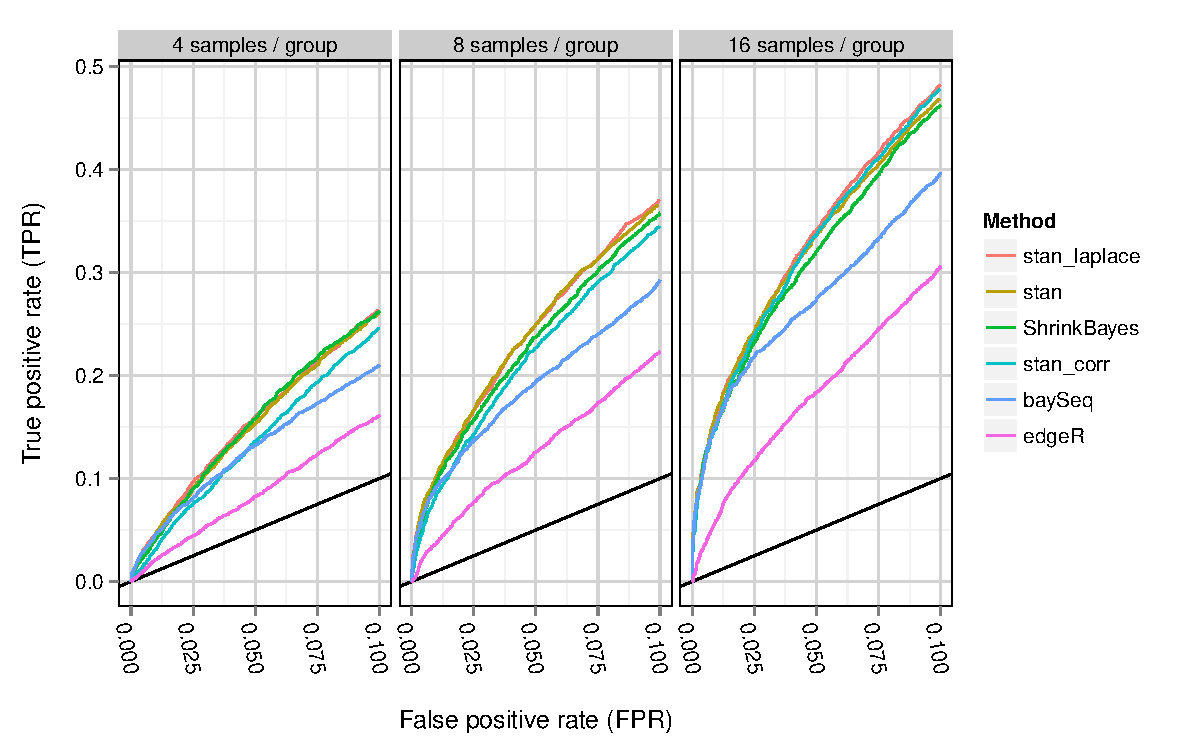
\includegraphics[width=\textwidth]{exampleROC0_1}}
\caption{Example ROC curves for false positive rates below 0.1 for the approaches using \citeauthor{ji2014estimation}, \edgeR{}, and \baySeq{} described in Section \ref{s:alternative}, the \ShrinkBayes{} approach described in Section \ref{s:shrinkbayes} and the eBayes approach described in Section \ref{s:ebayes} using both normal and laplace distributions for the half-parental difference and hybrid effect.}
\label{f:roc}
\end{figure}
The ROC curves indicate modest performance, e.g. for a false positive rate of 5\%, the best performing methods only achieved a true positive rate of just over 15\%. This is consistent with our expectation discussed in Section \ref{s:sim_data} due to the low signal-to-noise ratio in these simulated data. 

For this simulation, we can see that the approaches based on the model in Section \ref{s:model}, i.e. eBayes and \ShrinkBayes{}, provide the best true positive rate for a given false positive rate. Also, as expected, as the sample size increases, our ability to distinguish genes with EH from genes without improves. 

Figure \ref{f:auc} provides the area under the ROC curve (AUC) below a false positive rate of 0.1 across the 10 simulations for each of the 3 different sample sizes. 
\begin{figure}
\centerline{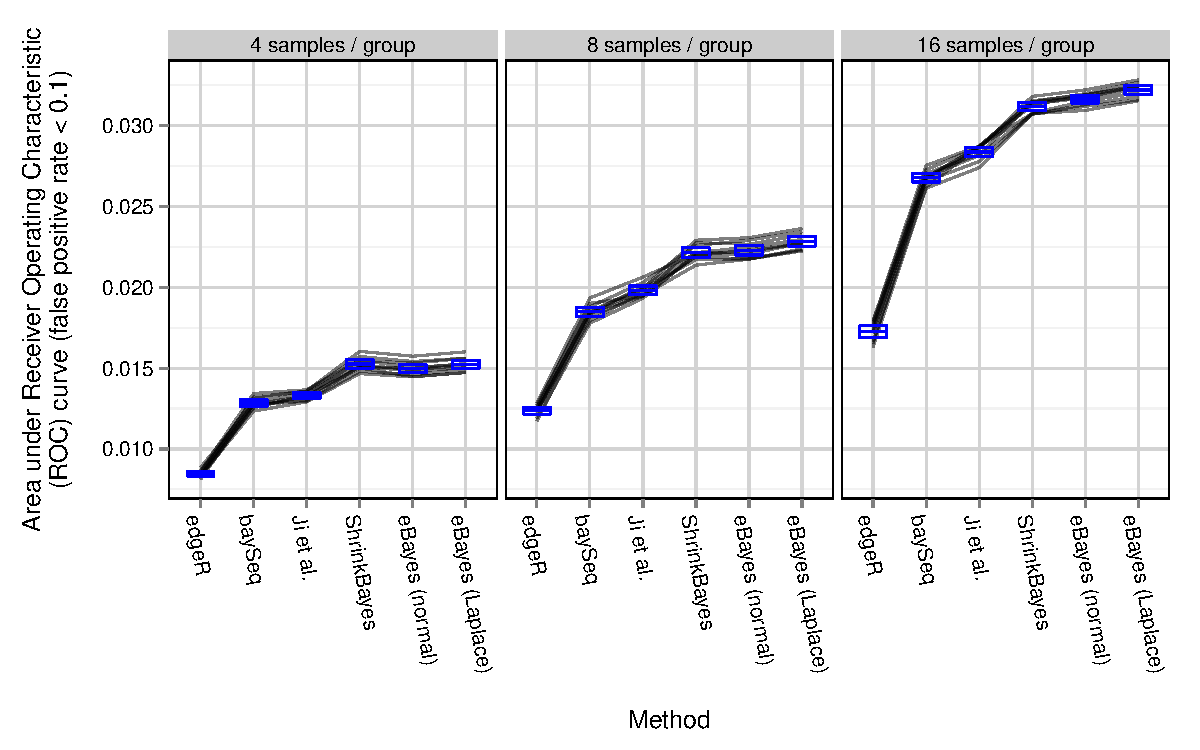
\includegraphics[width=\textwidth]{auc-facet-TRUE}}
\caption{Area under the ROC curves (AUC) below a false positive rate of 0.1 for 3 different replicates per variety for the approaches using \citeauthor{ji2014estimation}, \edgeR{}, and \baySeq{} as described in Section \ref{s:alternative}, the \ShrinkBayes{} approach described in Section \ref{s:shrinkbayes} and the eBayes approach described in Section \ref{s:ebayes} using both normal and laplace distributions for the half-parental difference and hybrid effect. Each line is a different simulation while the blue box indicates mean AUC (plus or minus one standard error).}
\label{f:auc}
\end{figure}
Similar to the single ROC curve, the eBayes and \ShrinkBayes{} methods appear to outperform the other methods in terms of AUC. This improvement ranges from about a 20\% improvement over Ji et al. to about a 100\% improvement over \edgeR{} (which was not designed for heterosis testing).

With 4 replicates per variety, there does not appear to be much of a difference between \ShrinkBayes{} and the eBayes approaches, but as the number of replicates increases, the eBayes approaches appear to improve relative to \ShrinkBayes{}. Two differences exist between the \ShrinkBayes{} and eBayes approaches that could explain the difference in AUC: 1) \ShrinkBayes{} utilizes a different empirical Bayes approach for estimating both the hyperparameters and the gene-specific parameters and 2) the measure of EH is slightly different due to INLA not providing a full posterior. 

There also appears to be a pattern of the eBayes (Laplace) systematically performing better than eBayes (normal). We suspect this is because the Laplace distributions are better approximations to the true underlying distribution for these parameters and we discuss this in Section \ref{s:discussion}.

\subsection{Hyperparameter estimation}

As described in Section \ref{s:simulation}, we simulated data only from the negative-binomial portion of the model, but not from the hierarchical distributions. Thus, there are no true values for the hyperparameters to compare against. But, we can compute means and standard deviations of the gene-specific parameters that were used in the simulation study and compare these to the estimated hyperparameter values. 
\begin{table}
\caption{Empirical values calculated from the gene-specific parameters used in the simulation and mean of estimated values across the 10 simulations within replicate number. Maximum standard deviation in the estimates across the 10 simulations was 0.004.}
\label{t:hyperparameter}
\begin{tabular}{l|r|rrr|}
& \multicolumn{1}{c|}{Empirical} & \multicolumn{3}{c}{\# of replicates}\\
Parameter & value & 4 & 8 & 16 \\
\hline
% with (SD)
% $\eta_\phi$ & 4.675 & 4.681 (0.004) & 4.741 (0.002) & 4.817 (0.003) \\
% $\eta_\alpha$ & -0.017 & -0.023 (0.002) & -0.018 (0.003) & -0.014 (0.002)  \\
% $\eta_\delta$ & -0.046 & -0.046 (0.002) & -0.031 (0.002) & -0.022 (0.003)  \\
% $\eta_\phi$ & -2.713 & -2.290 (0.004) &  -2.335 (0.003) & -2.387 (0.002)\\
% \hline
% $\sigma_\phi$ & 1.815 & 1.821 (0.002) & 1.779 (0.002) & 1.726 (0.003)\\
% $\sigma_\alpha$ & 0.364 & 0.459 (0.002) & 0.399 (0.002) & 0.357 (0.002) \\
% $\sigma_\delta$ & 0.145 & 0.389 (0.002) & 0.317 (0.002) & 0.268 (0.001) \\
% $\sigma_\psi$ & 0.737 & 0.401 (0.001) & 0.493 (0.001) & 0.542 (0.001) \\
% 3 decimal places
% $\eta_\phi$ & 4.675 & 4.681 & 4.741  & 4.817  \\
% $\eta_\alpha$ & -0.017 & -0.023  & -0.018 & -0.014  \\
% $\eta_\delta$ & -0.046 & -0.046 & -0.031  & -0.022   \\
% $\eta_\phi$ & -2.713 & -2.290  &  -2.335  & -2.387\\
% \hline
% $\sigma_\phi$ & 1.815 & 1.821  & 1.779  & 1.726 \\
% $\sigma_\alpha$ & 0.364 & 0.459  & 0.399  & 0.357  \\
% $\sigma_\delta$ & 0.145 & 0.389  & 0.317  & 0.268  \\
% $\sigma_\psi$ & 0.737 & 0.401 & 0.493 & 0.542 \\
$\eta_\phi$ & 4.7\phantom{00} & 4.7\phantom{00} & 4.7\phantom{00}  & 4.8\phantom{00}  \\
$\eta_\alpha$ & -0.017 & -0.023  & -0.018 & -0.014  \\
$\eta_\delta$ & -0.046 & -0.046 & -0.031  & -0.022   \\
$\eta_\phi$ & -2.7\phantom{00} & -2.3\phantom{00}  &  -2.3\phantom{00}  & -2.4\phantom{00} \\
\hline
$\sigma_\phi$ & 1.8\phantom{0} & 1.8\phantom{0}  & 1.8\phantom{0}  & 1.7\phantom{0} \\
$\sigma_\alpha$ & 0.36 & 0.46  & 0.40  & 0.36  \\
$\sigma_\delta$ & 0.15 & 0.39  & 0.32  & 0.27  \\
$\sigma_\psi$ & 0.74 & 0.40 & 0.49 & 0.54 \\
\hline
\end{tabular}
\end{table}
Table \ref{t:hyperparameter} provides the computed means and standard deviations from the gene-specific parameter values, called empirical values, and compares these values against the mean of estimated hyperparameters across the 10 simulations within replicate number. For the mean parameters, there is reasonable agreement amongst the different numbers of replicates with a somewhat high estimate for the mean of the overdispersion parameter $(\eta_\phi)$ and, perhaps, a trend for the mean of the hybrid effect ($\eta_\delta$), although we would not have expected this. For the standard deviation parameters, $\sigma_\phi$ is consistent across the replicate numbers, $\sigma_\alpha$ and $\sigma_\delta$ mean estimates are decreasing toward the empirical values as the number of replicates increases, and $\sigma_\phi$ is increasing toward the empirical value as the number of replicates increases. %We expect this pattern for $\sigma_\alpha$ and $\sigma_\delta$ since these are based on moment matching of independent gene-specific parameter estimates. For low numbers of replicates, these independent estimates will have relatively large sampling variability that will cause a bias toward larger values for the moment-matched standard deviation estimates.



\section{Searching for gene expression heterosis in the maize experiment}
\label{s:maize}

We used our method to analyze a maize data set \citep{paschold2012complementation} of \RNAseq{} gene expression in parental lines B73 and Mo17 and the hybrid genotype (B73$\times$Mo17) with a total of 39,656 genes. Each variety had four biological replicates measured with Illumina methodology and equipment. Reads were mapped to the whole reference genome using the short reads aligner, NOVOALIGN. For more specifics, please see \cite{paschold2012complementation}. 

We analyzed the data using all the methods compared in the previous section. The computation time on a desktop with two 4-core 3.6GHz Intel Xeon processor was 14 seconds for \edgeR{}, 1.3 minutes for \citeauthor{ji2014estimation}, 10 hours for the eBayes approaches, and 17 hours for \baySeq{}. In the eBayes approach, the vast majority of the time is spent on independent MCMC analysis for each gene. Thus we parallelized this step using {\tt doMC} \citep{revolution2014domc} and {\tt plyr} \citep{hadley2011split}. When parallelized across 5 cores, the eBayes approaches took about 2.5 hours. ShrinkBayes took 12 hours on a cluster node with two 8-core 2.6GHz Intel Haswell E5-2640 v3 processors where the code was also parallelized across 5 cores.

For the eBayes (Laplace), we estimated the hyperparameters to be $\hat{\eta}_\phi = 3.44$, $\hat{\sigma}_\phi = 2.74$, $\hat{\eta}_\alpha = -0.05$, $\hat{\sigma}_\alpha=0.36$, $\hat{\eta}_\delta = 0.08$, $\hat{\sigma}_\delta=0.33$, $\hat{\eta}_\psi = -2.35$, and $\hat{\sigma}_\psi=0.60$. We then performed independent MCMC analysis for each gene conditional on these hyperparameters. As with the simulation study, we ran 4 chains simultaneously and doubled the number of MCMC iterations until each gene-specific parameter had an effective sample size above 1,000. 

Figure \ref{f:gene_specific_estimates} provides point estimates of the gene-specific parameters from the initial \edgeR{} estimation step and after the eBayes (Laplace) procedure described in Section \ref{s:ebayes}. 
\begin{figure}
\centerline{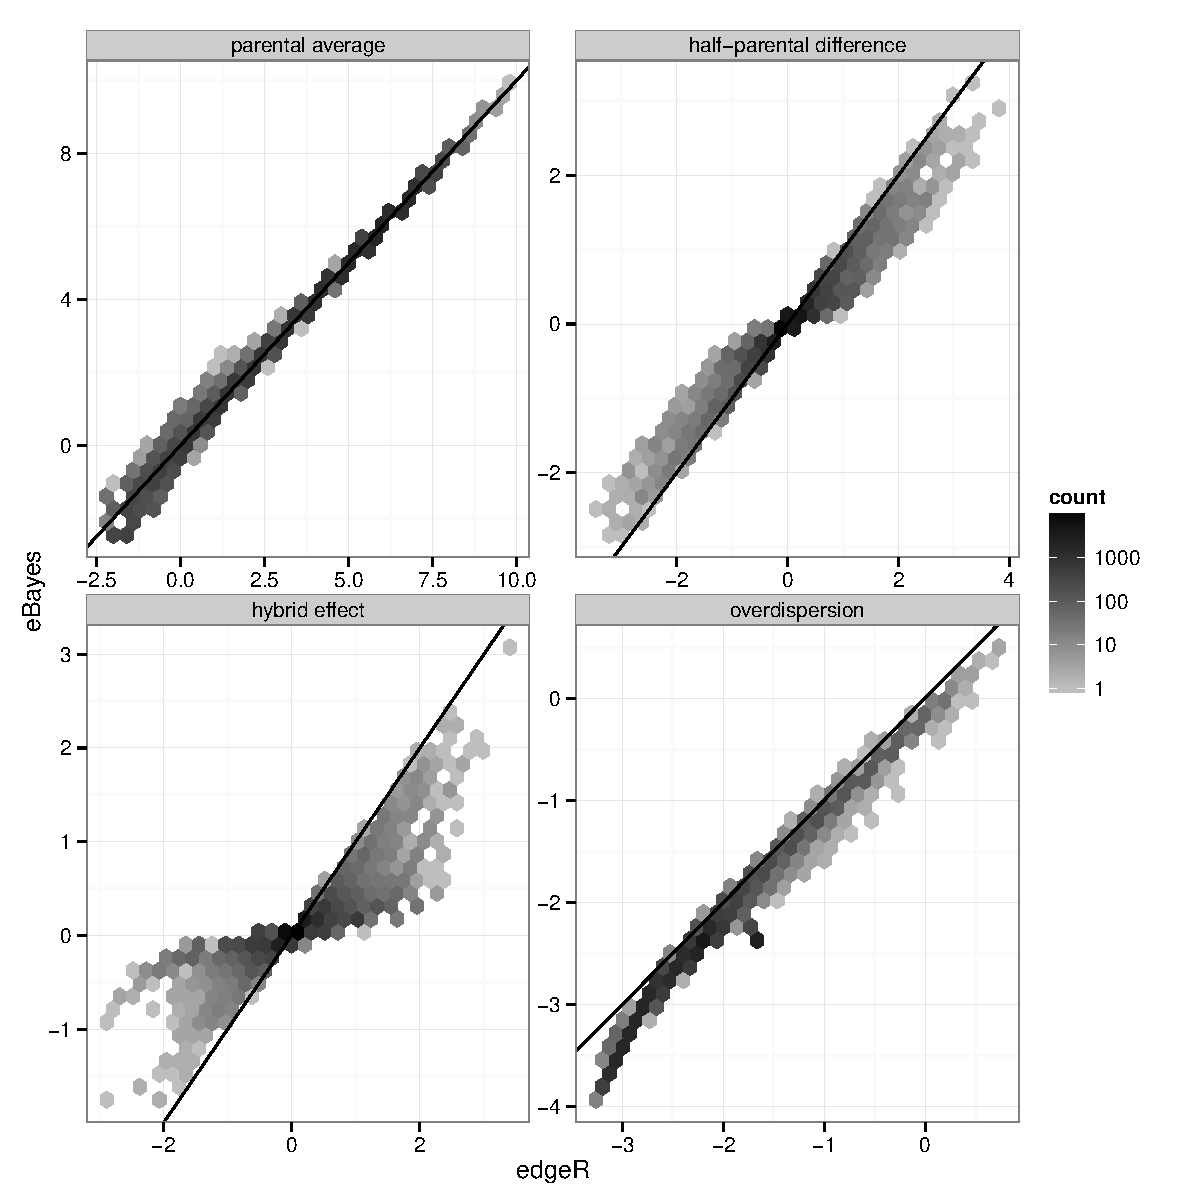
\includegraphics[width=\textwidth]{gene_specific_estimates.pdf}}
\caption{Two-dimensional histogram of point estimates from \edgeR{} and posterior means from eBayes (Laplace) along with the $y=x$ diagonal.}
\label{f:gene_specific_estimates}
\end{figure}
This figure shows shrinkage for large absolute values of $\alpha$ and $\delta$ from the \edgeR{} estimation toward $\hat{\eta}_\alpha$ and $\hat{\eta}_\delta$ which are both approximately zero. The figure also shows decreased values for the overdispersion parameter with larger decreases for high and low values of overdispersion. Finally, very little, if any, shrinkage is observed for $\phi$. 

With posteriors for all parameters, we can calculate empirical Bayes posterior probabilities for LPH and HPH. For each gene, the quantity of interest is likely to be the maximum of these two probabilities. For each gene with a high probability of either HPH or LPH, the magnitude of the effect is of interest, thus we calculate 
\begin{equation}
% \mbox{estimated effect size}_g = \left\{ 
% \begin{array}{ll}
% \hat{\mu}_{g3} - \min(\hat{\mu}_{g1},\hat{\mu}_{g2}) & \mbox{if } \hat{\mu}_{g3} < \min(\hat{\mu}_{g1},\hat{\mu}_{g2}) \\
% \hat{\mu}_{g3} - \max(\hat{\mu}_{g1},\hat{\mu}_{g2}) & \mbox{if } \hat{\mu}_{g3} > \max(\hat{\mu}_{g1},\hat{\mu}_{g2}) \\
% 0 & \mbox{otherwise},
% \end{array} 
% \right. 
\mbox{estimated effect size}_g \equiv \left\{ 
\begin{array}{ll}
\hat{\delta}_g - |\hat{\alpha}_g| & \mbox{if } \hat{\delta}_g > \phantom{-}|\alpha_g| \\
\hat{\delta}_g + |\hat{\alpha}_g| & \mbox{if } \hat{\delta}_g < -|\alpha_g| \\
0 & \mbox{otherwise},
\end{array}.
\right. 
\label{e:effect_size}
\end{equation}
This estimated effect size is the difference between hybrid mean and the nearest parent with negative values indicating LPH and positive values indicating HPH. If the hybrid mean is estimated to be between the parents, this effect is defined to be zero. 


Figure \ref{f:volcano} provides a volcano plot, in this case a bivariate histogram, to visualize the maximum of the probabilities of LPH and HPH versus estimated effect size. 
\begin{figure}
\centerline{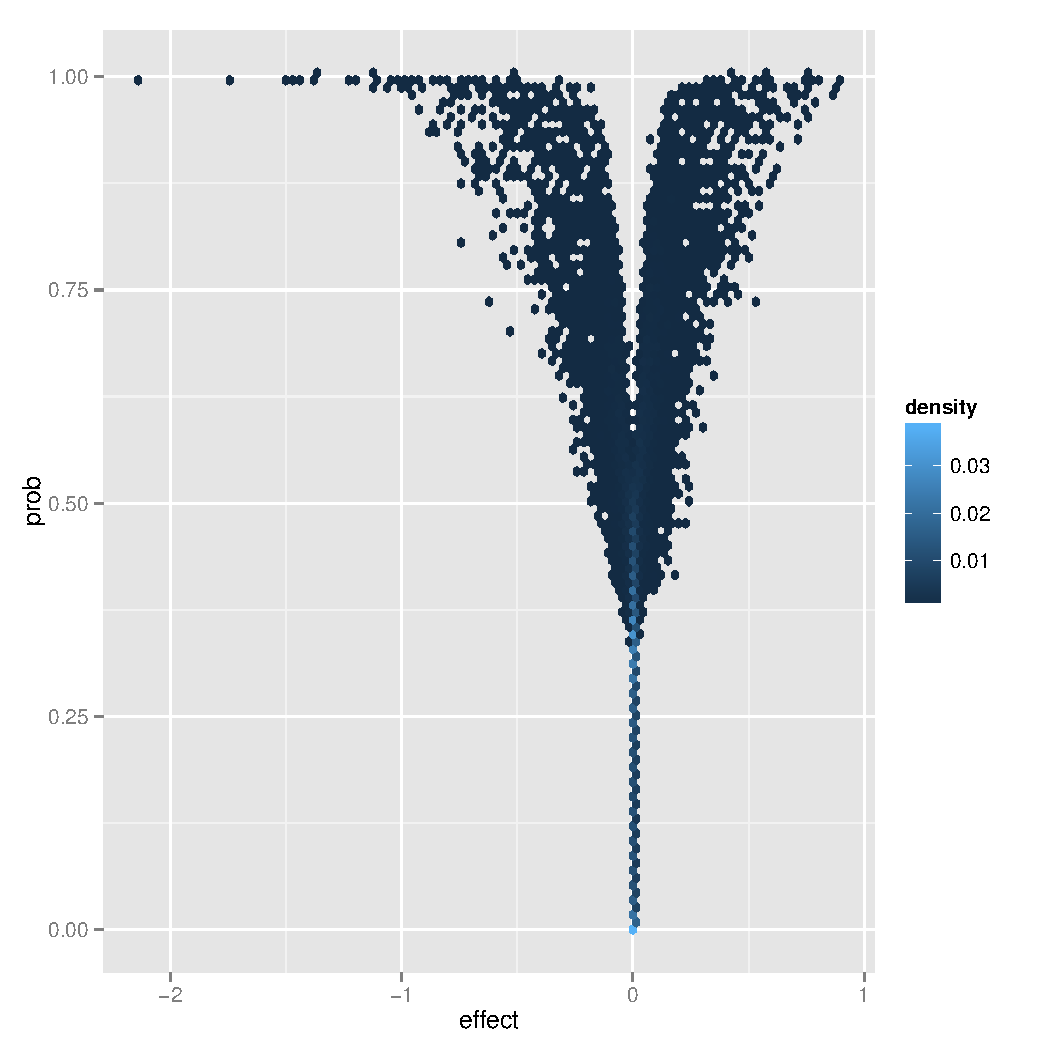
\includegraphics[width=\textwidth]{volcano}}
\caption{A bivariate histogram of the maximum of the LPH and HPH probabilities versus estimated effect size defined in equation \eqref{e:effect_size} for the B73 $\times$ Mo17 maize experiment using eBayes (Laplace).}
\label{f:volcano}
\end{figure}
The figure shows a ridge at an effect size of zero for probabilities below 0.5. Above a probability of 0.5, we see a prototypical volcano pattern, with increased EH probability corresponding to larger estimated effect sizes and no estimated effect sizes near zero for genes with high EH probability. We also see asymmetry, with larger negative effect sizes than positive effect sizes due to genes with hybrid counts near zero and relatively high parental counts. Genes with high estimated posterior probabilities of EH and large estimated effect sizes are candidates for further investigation.






\section{Discussion}
\label{s:discussion}

Geneticists speculate that gene expression heterosis is one possible explanation of phenotypic heterosis of traits, such as plant height or grain yield. Existing methods for identifying differential gene expression based on \RNAseq{} data are not directly applicable for detecting heterosis genes. \cite{ji2014estimation} introduced an empirical Bayes approach based on a hierarchical model for microarray data. We followed their approach, modified to allow for \RNAseq{} read counts as measures of transcript abundance. We developed an empirical Bayes approach based on obtaining estimates for hyperparameters followed by MCMC to estimate gene-specific parameters. The empirical Bayes posteriors can be used to estimate posterior probabilities of high and low parent heterosis. Through a simulation study, we demonstrated that this method outperformed alternative methods, and performed comparably well with a similar model in \ShrinkBayes{}, which estimates the posterior via INLA. We then demonstrated the use of the methodology on a maize experiment in which phenotypic heterosis is well known. 

Although our method appears to hold some advantage over existing methods, we believe our approach can be improved by refining the hierarchical model for the gene-specific parameter distribution. Figure \ref{f:scatterplot} shows marginal and bivariate histograms for eBayes (Laplace) posterior means for the gene-specific parameters. 
\begin{figure}
\centerline{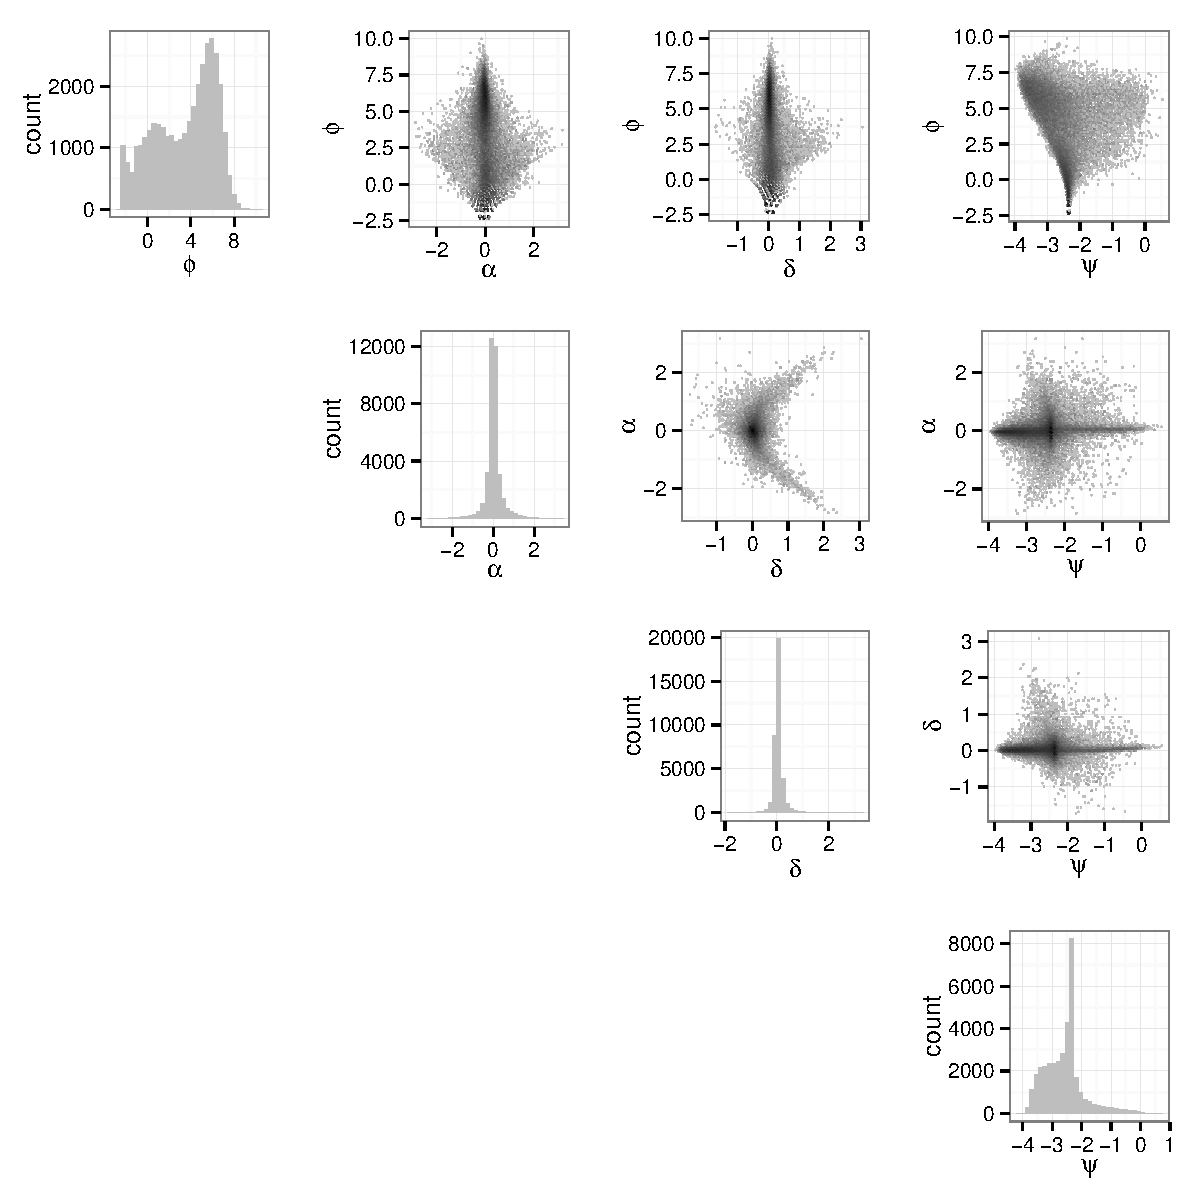
\includegraphics[width=\textwidth]{estimates}}
\caption{Marginal and bivariate histograms of posterior means for gene-specific parameters for the B73 $\times$ Mo17 maize experiment.}
\label{f:scatterplot}
\end{figure}
These figures show markedly departures from marginal model assumptions, e.g. normality assumptions for $\phi_g$ and $\psi_g$, and independence assumptions for $(\phi_g,\psi_g)$ and $(\alpha_g,\delta_g)$. The plot of $\phi_g$ versus $\psi_g$ shows a pattern where the mean overdispersion decreases as the mean expression level increases. The plot of $\alpha_g$ versus $\delta_g$ shows a rotated V pattern where $\delta_g$ appears to be equal to $|\alpha_g|$. This V pattern is consistent with Mendel's Law of Dominance where the hybrid has mean expression equal to the parent with higher mean expression. 

In addition to improving the hierarchical distribution, we believe better estimates of the parameters of this distribution, i.e. the hyperparameters, will also improve detection of gene-expression heterosis. Our current method, based on moment matching of essentially independently estimated gene-specific parameters, provides consistent estimators as the number of replicates per variety increases. But typically the number of replicates per variety is quite small. In our data there are only four replicates per variety, and therefore asymptotic justifications are deficient. There are a variety of alternative estimation approaches to explore, e.g. expectation-maximization algorithms or fully Bayesian approaches.

Notwithstanding these improvements, we believe our approach is a computationally efficient method that can immediately aid scientists who are interested in identifying candidate genes involved in a genetic mechanism of heterosis. 

This paper has focused on statistical methods for detecting EH in gene expression using RNA-seq data.  EH at the transcript level is only one of multiple molecular genetic mechanisms that may play roles in establishing hybrid vigor.  Complementation \citep{paschold2012complementation}, allele-specific expression \citep{bell2013rna,wei2013computational}, and other complex forms of genomic and epigenetic interaction \citep{chen2013genomic} are all plausible as mechanisms partially responsible for phenotypic heterosis.  Further study of these phenomena using modern genomic technologies and appropriate statistical methods should enhance our understanding of hybrid vigor.



\backmatter %  Please keep this command in your document in this position 

\if0\blind{
\section*{Acknowledgements}

The authors thank Andrew Lithio for help in implementing our model in \ShrinkBayes{}. Research reported in this publication was supported by National Institute of General Medical Sciences of the National Institutes of Health under award number R01GM109458. The content is solely the responsibility of the authors and does not necessarily represent the official views of the National Institutes of Health.
} \fi

%  If your paper refers to supplementary web material, then you MUST
%  include this section!!  See Instructions for Authors at the journal
%  website http://www.biometrics.tibs.org

%\section*{Supplementary Materials}
%The supplementary materials include three plain text files: the maize experiment data ({\tt data.csv}), a script to run our method ({\tt script.R}) on this data, and the \Stan{} model ({\tt model.stan}).  

\bibliography{jarad}
\bibliographystyle{biom}

% \appendix
% %  To get the journal style of heading for an appendix, mimic the following.
% \section{}
% \subsection{Material here}

\label{lastpage}

\end{document}
